\documentclass[11pt,a4paper]{article}
\usepackage[utf8]{inputenc}
\usepackage{amsmath}
\usepackage{amsfonts}
\usepackage{xcolor}
\usepackage{array}
\usepackage{amssymb}
%\usepackage{colortbl}
\usepackage{listings}
\usepackage{hyperref}
\usepackage{graphicx}

\newcommand{\boxgreen}{\colorbox{green}{\color{black}done}}
\newcommand{\boxyellow}{\colorbox{yellow}{\color{black}in progress}}
\newcommand{\boxred}{\colorbox{red}{\color{black}NYI}}

\newcommand{\pack}[1]{$>$ #1.java \newline}

%\newcommand{\tabID2}[2]  {\small \textit{Tabel \tabID : #2} \\ \normalsize}

% Counter for the requirements
\newcounter{reqc} 
\newcommand{\reqID} {%
   \stepcounter{reqc}%
   \thereqc}

% Counter for the figures/images
\newcounter{figc}
\newcommand{\figID} {%
   \stepcounter{figc}%
   \thefigc}
   
% Counter for the tables
   \newcounter{tabc}
\newcommand{\tabID} {%
   \stepcounter{tabc}%
   \thetabc}


\author{David Sverdlov \\ dsverdlo@vub.ac.be}
\title{Bachelorproef AMuRate: Project Plan 3e Bachelor Computerwetenschappen}
\begin{document}
% Begin title page
\begin{flushleft}
\noindent 
\includegraphics[width=0.6\linewidth]{Pictures/vub_logo.jpg} 
\end{flushleft}
{\let\newpage\relax\maketitle} % don't let it set newpage

\begin{center}

\includegraphics[width=4cm]{Pictures/amr_gold_thick.png} 
\end{center}



\newpage
\tableofcontents

\newpage
\section{Inleiding}
	\subsection{Doel}
De uitdaging van dit bachelorproject is om een applicatie te ontwikkelen voor het mobiele platform Android. De applicatie moet gebruikers in staat stellen om muzieknummers op te zoeken en een beoordeling te kunnen geven. Die scores worden dan opgestuurd naar een data-collection server met een database, waar later recommendeer algoritmen op zullen werken. (De implementatie daarvan valt niet binnen de scope van dit project.) \\
De promotor van dit project is Dr. Peter Vranckx en wordt geassisteerd door Maarten Deville.

	\subsection{Projectbeschrijving}
	
Gebruikers moeten eerst en vooral muziek kunnen opzoeken. Hier zal een scherm voor zorgen, waar men de zoekgegevens kan invullen. Er is een veld voor de titel van een lied in te vullen, en een veld voor de artiest- of groepsnaam. Beide velden hoeven niet tesamen ingevuld te zijn, het volstaat dat er maar een veld ingevuld is. Er zal een melding gegeven worden wanneer er op de zoek-knop geduwd werd zonder dat er iets van zoekgegevens werd opgegeven.
\\ 

Een hulp-knop informeert mensen over het (correct) gebruik van de applicatie. Dit gebeurt door een pop up en kan gesloten worden door op OK te klikken. 
\\ 
 
Wanneer er geen werkende data connectie is, zij dat de data-connectie niet aan staat, of dat er geen beschikbaar netwerk in de buurt is, zal de gebruiker een melding krijgen dat hij een werkende data verbinding nodig heeft eer informatie gedownloaded kan worden. 
\\ 
	
Wanneer een gebruiker beschikt over een actieve data verbinding en minstens één zoekterm ingevuld heeft, zal de applicatie een HTTP GET oproep doen naar een grote externe database met muziekgegevens. Die database is die van Last.fm. Op het scherm zal een indicator tevoorschijn komen dat er een oproep behandeld wordt. Eens aangekomen, zal de Last.fm API de oproep analyseren en een antwoord vormen met de opgevraagde informatie. Eens dat antwoord bij de applicatie aagekomen is, zal de applicatie het resultaat van de oproep aan de gebruiker tonen. Zie hoofdstuk GUI voor een visueel voorbeeld van dit proces. 
\\ 
	
Wanneer men kiest om de resultaten te bekijken, wordt er een lijst getoond met alle opties. Door op een van de resultaten te klikken, kan er naar het volgende scherm gegaan worden: een gedetailleerde pagina met meer informatie dan de beknopte optie waarop geklikt werd. 
\\ 
	
De gebruiker kan liedjes zoeken door het 'title' veld in te vullen, maar ook artiesten/groepen opzoeken door enkel iets in het 'artiest' veld te schrijven. Wanneer de gebruiker enkel op artiest zoekt, gaan de gevonden resultaten doorverwijzen naar een gedetailleerde artiesten pagina. Op dit scherm is een kleine biografie te lezen van de artiest, een link naar een wiki-pagina, een afbeelding en een lijst van de top tracks en top albums van die artiest. De gebruiker kan scrollen in beide lijsten en op elke item klikken om naar de respectievelijke gedetailleerde pagina's te gaan.
\\

Het gedetailleerde scherm van een lied geeft wat triviale informatie over het lied in kwestie, zoals de duratie, albumnaam, artiestnaam, ... Daarnaast nog een afbeelding van het album\footnote{Indien er een afbeeldings URL beschikbaar is, anders een standaard blanco afbeelding.}. Indien er meer album informatie beschikbaar is, zal er een knop zijn, waar gebruikers op kunnen klikken om naar de gedetailleerde pagina voor een album te gaan. 
\\ 	
Op het track scherm is er een deel van de pagina bedeeld aan het score systeem. Naast de mogelijkheid om zelf eenmalig een score te geven (tussen 0 en 5, met stappen van een halve precisie), wordt ook de gemiddelde score weergegeven van alle scores voor dat lied (en het aantal scores waar het gemiddelde van berekend werd). Een boodschap informeert de gebruiker of hij al een score heeft gegeven voor dat lied, en wat die score was indien zo. Als er geen verbinding gemaakt kan worden, zal dit ook genotifieerd worden. 
\\ 
	
Het gedetailleerde scherm voor een album toont enkele informatieve zaken van het album en alle liedjes erin. De gebruiker kan op elk lied klikken om naar het scherm te navigeren met meer informatie en/of een score te geven. Met een X-knop kan er terug gegaan worden naar het hoofdmenu.
\\ 
	
Wanneer een score toegediend wordt en er een werkende data verbinding is, moet de score niet alleen in de lokale database toegevoegd worden, maar ook naar de server gestuurd worden. De scores worden kunnen geidentificeerd worden via hun MBID en in de externe database worden ze opgeslagen met een unieke Android device nummer van het GSM toestel. 
\\
Vanaf het beginscherm kan de gebruiker ook op de knop 'History' klikken om zijn geschiedenis te bekijken. Op het geschiedenis scherm zijn er vanboven 3 tabs te zien: 'Search', 'Tracks' en 'Ratings'.  De tabs staan in een horizontale scrollview (er kunnen dus makkelijk bijgezet worden). De geschiedenis wordt dus onderverdeeld in zoekgeschiedenis (opgegeven zoektermen), trackgeschiedenis (bekeken tracks) en rating geschiedenis die alle gegevens scores bijhoudt. Elke onderverdeling heeft de optie om zijn geschiedenis te wissen.
	
	
	\subsection{Afkortingen en definities}
		\subsubsection{API}
		API staat voor Application Programming Interface en zorgt voor de communicatie tussen programmas, door de scheiding te vormen tussen verschillende lagen van abstracties.
		\subsubsection{XML/JSON}
		XML staat voor Extensible Markup Language en is een van de meest gebruikte opmaaktalen, die gestructureerde gegevens kunnen omzetten in platte tekst. (Om het zo makkelijk(er) door te kunnen sturen.)
		\newline
		JSON is aan afkorting van JavaScript Object Notation en is een alternatieve simpele manier om objecten voor te stellen als platte tekst.
		\subsubsection{HTTP}
		HTTP staat voor HyperText Transfer Protocol en is het medium tussen een webbrowser en een webserver. Die communicatie gebeurt door middel van URLs, die verwijzen naar 'iets' op een of andere webserver.
		\subsubsection{GUI}
		GUI staat voor Graphical User Interface en is een visuele vormgeving van een programma, dat door middel van knoppen, afbeeldingen, ... gebruikers toelaat om op een gebruiksvriendelijkere manier met de applicatie om te gaan .
		
		\subsection{MBID}
		MBID staat voor MusicBrainz Identifier. MusicBrainz is een grootschalige onderneming die een universeel, uniek muziek identificerings systeem implementeert. Een ID bestaat uit 36 karakters en kan gebruikt worden voor liedjes, artiesten, albums,...

\section{Achtergrond}
	\subsection{Last.fm/API: REST}
Om informatie (over muziek in dit geval) op te kunnen zoeken, moet er gebruik gemaakt worden van een online database met een openbare en hanteerbare API. \textit{Last.fm} is een muziek recommendation service met een enorme online muziek database, die  een gratis (lees: voor geregistreerde gebruikers) API aanbiedt, die iedereen toelaat om mobiele/desktop programmas of web services te bouwen met hun data.
\newline
Die procedure verloopt als volgt: om data uit de database te halen moet er een call (oproep) gestuurd worden. Deze gebeurt via HTTP GET naar de Last.fm server die op zijn beurt antwoordt met een XML object (of JSON op aanvraag). De architectuur van client$<->$server die hier gebruikt wordt heet 'REST(ful)'. 
\newline
De link van de aanvraag wordt opgebouwd uit 3 delen$;$ de basis van de API, de methode en de api-key. Een api-key is te verkrijgen door te registeren bij Last.fm. De basis is altijd 'ws.audioscrobbler.com/2.0/' en de methode van de vorm '?method=category.function'. 
De API biedt tientallen methodes aan, zoals bijvoorbeeld artist.search, artist.getTopAlbums, artist.getTopTracks, track.getInfo, track.search, track.getTags, album.search, album.getBuyLinks, ... . 
\\
De 'x.search' en 'x.getInfo' oproepen zullen het meeste gebruikt worden in dit project. 

	\subsection{REST architectuur}
	REST staat voor Representational State Transfer en is een type van architectuur voor bepaalde gedistribueerde systemen (zoals het World Wide Web), waarin een duidelijke onderscheiding wordt gemaakt tussen client en server. Clienten kunnen oproepen doen naar de server, die de oproepen analyseert, een antwoord formuleert, en dat antwoord terug naar de klant stuurt. REST maakt gebruik van werkwoorden en zelfstandige naamwoorden om de oproepen ook leesbaar voor mensen te maken. De standaard werkwoorden zijn GET, POST, PUT en DELETE, om data te kunnen verkrijgen, wijzigen of opsturen.
	
	\subsection{Website en repository}
		Voor dit project werd er gebruik gemaakt van Git als versiebeheersysteem, omdat het een gratis, eenvoudige en betrouwbare manier is om de broncode te beheren. Om updates in het project naar de repository te sturen wordt er gebruikt gemaakt van Github voor Windows. Nog een voordeel van deze dienst is dat Github de mogelijkheid biedt om snel en simpel websites te maken voor de bestaande projecten. Zo werd er een kleine website voor dit project opgesteld, die terug te vinden is op: \url{http://dsverdlo.github.com/AMuRate/}. Hier kan men de open-source broncode bekijken, het logboek of dit document raadplegen en de applicatie (.apk) downloaden voor Android 4.0+ toestellen. (Zie sectie Technische Details voor meer informatie over het installeren)
		
	\subsection{Naam en logo}
		De naam van een project geeft meestal een kleine beschrijving van wat de applicatie doet/waar hij voor dient. AMuRate komt van 'Android Music Rating'. Omdat het project vooral geïmplementeerd zou worden via een Android emulator en simpelweg 'AMR' te kort en onduidelijk zou zijn, werd er gekozen voor AMuRate. Het logo (zoals te zien op de voorpagina) is een compositie van een 5-ster in een bol die iets weg heeft van een 'dragonball' (uit de Japanse animatieserie DragonBall Z). In DBZ bestaan er maar 7 bollen op de hele wereld en wanneer die allemaal verzameld zijn, mag de beheerder een wens doen. Een beetje gelijkaardig aan hoe elke artiest hoopt 5 sterren (/ 7 dragon balls) te verzamelen. 
	In de ster zelf zijn drie gekleurde letters (AMR) te onderscheiden, naar de naam van de applicatie.
	
	
%\newpage % hack for layout	
\section{Vereisten}
Hieronder volgt een tabel die alle vereisten opsomt, met hun geimplementeerde status. Deze tabel werd in de loop van het project up-to-date gehouden met verschillende statuskleuren, naargelang de level van afwerking per vereiste. Momenteel zijn ze allemaal groen omdat elke onderstaande functionaliteit geimplementeerd is.

	% Get a nice table with colors running here, bro
	\begin{tabular}{| l | l | c | r |}
	\hline
	ID 		& 	Side	&	Beschrijving						& Status 		\\ \hline \hline
	\reqID	&	Client	&	Titel en artiest kunnen invullen	& \boxgreen 	\\ \hline
	\reqID 	&	Client	&	Enkel op titel zoeken				& \boxgreen		\\ \hline
	\reqID	& 	Client	&	Enkel op artiest opzoeken 			& \boxgreen		\\ \hline
	\reqID 	& 	Client	&	Gedetailleerd lied weergeven		& \boxgreen 	\\ \hline
	\reqID 	& 	Client	&	Gedetailleerd artiest weergeven		& \boxgreen 	\\ \hline
	\reqID 	& 	Client	&	Gedetailleerd album weergeven		& \boxgreen 	\\ \hline
	\reqID	& 	Client	&	Scores beheren in lokale database	& \boxgreen  	\\ \hline
	\reqID	& 	Client	&	Geschiedenis beheren in database	& \boxgreen  	\\ \hline
	\reqID	& 	Client	&	Geschiedenis weergeven op scherm	& \boxgreen  	\\ \hline
	\reqID	& 	Server	&	Scores opsturen naar externe db		& \boxgreen		\\ \hline
	\reqID	&	Server	&	Scores ophalen uit externe db		& \boxgreen		\\ \hline
	\reqID	& 	Server	& 	Multithreading op de server			& \boxgreen		\\ \hline
	\reqID	& 	Both	& 	Ongesyncte scores naar ext. db		& \boxgreen		\\ \hline
	\reqID	&	Both	&	Check of er al een score bestaat	& \boxgreen		\\ \hline
	
%	\reqID	& 	necessity	&			& \boxred 		\\ \hline
%	\reqID	&	optional	&	Stream$/$preview 30sec songs		& \boxyellow 	\\ \hline
%	\reqID	&	optional	&	Caching implementeren				& \boxred 		\\ \hline
%	\reqID 	& 	optional	&	Onderzoek uitbreidbaarheid (ios?)	& \boxred 		\\ \hline
%	\reqID 	&	optional	&	Informatie ophalen van media speler & \boxred 		\\ \hline
	%\hline	
	\end{tabular} \\ \newline
	\small \textit{Tabel \tabID : Vereisten van het project met uitleg en implementatiestatus.} \normalsize
	\\ \newline
	Zoals in de projectbeschrijving reeds gezegd werd, bestaat het project uit twee afzonderlijke delen, die verbonden kunnen worden door een internetverbinding. Aan de client-kant is er de applicatie op Android, en aan de server-kant een data-collection server die scores verzameld en geregeld gebruikt voor recommendeer algoritmen. De server-kant is een kleiner pakket dan de client-kant, maar niet minder belangrijk. 
	\\ \newline

	% text?


%\newpage % hack for layout	
	%%%%%%%%%%%%%%%%%
	% Implementatie %
	%%%%%%%%%%%%%%%%%
\section{Implementatie}
	\subsection{Android applicatie}
		\normalsize  
		De broncode van het project is opgedeeld in 3 packages: \textit{gui, objects en services}. Hier een voorlopig overzicht van de packages en hun inhoud:\\
		
		 \textbf{com.dsverdlo.AMuRate.gui} \newline		
		 \pack{AlbumActivity}
		 \pack{AnimationView}
		 \pack{ArtistActivity}
		 \pack{HistoryActivity}
		 \pack{MainActivity}
		 \pack{SearchArtistActivity}
		 \pack{SearchResultsActivity} 
		 \pack{TrackActivity}
		 
		\textbf{com.dsverdlo.AMuRate.objects} \newline
		\pack{Album}
		\pack{AMuRate}
		\pack{Artist}
		\pack{History}
		\pack{Rating}
		\pack{Track}
		
		\textbf{com.dsverdlo.AMuRate.services} \newline
		\pack{DatabaseSyncer}
		\pack{ExternalDatabaseConnect}
		\pack{HttpConnect}
		\pack{InternalDatabaseHistoryAdapter}
		\pack{InternalDatabaseManager}
		\pack{InternalDatabaseRatingAdapter}
		
		 In het \textit{GUI} package zitten alle activities\footnote{Dit is de naam van een scherm in Android} en alle klassen die te maken hebben met het uiterlijk van de applicatie. Elk scherm om iets op weer te geven heeft een eigen activity nodig. \\
		In het \textit{objects} package zitten de objecten/units/simpele java klassen, die abstractie brengen in het project. Het is ook hier dat de globale applicatie 'AMuRate.java' zit, die gebruikt wordt om een soort van globale Android variabelen te kunnen gebruiken.  \\
		Package \textit{services} bevat de klassen die instaan voor verschillende diensten die moeten gebeuren in de applicatie. Zo is er de HttpConnect klasse, die de oproepen doet en antwoorden download van de Last.fm API en afbeeldingen per http binnenhaalt. De InternalDatabaseManager klasse is ook een dienst die verleend wordt aan de interne database.

	\subsection{Data flow}
	Om de overgangen tussen alle schermen overzichtelijk te illustreren, werd er een DFD\footnote{Data Flow Diagram} gemaakt. Zie onderstaande afbeelding: \newline
	
	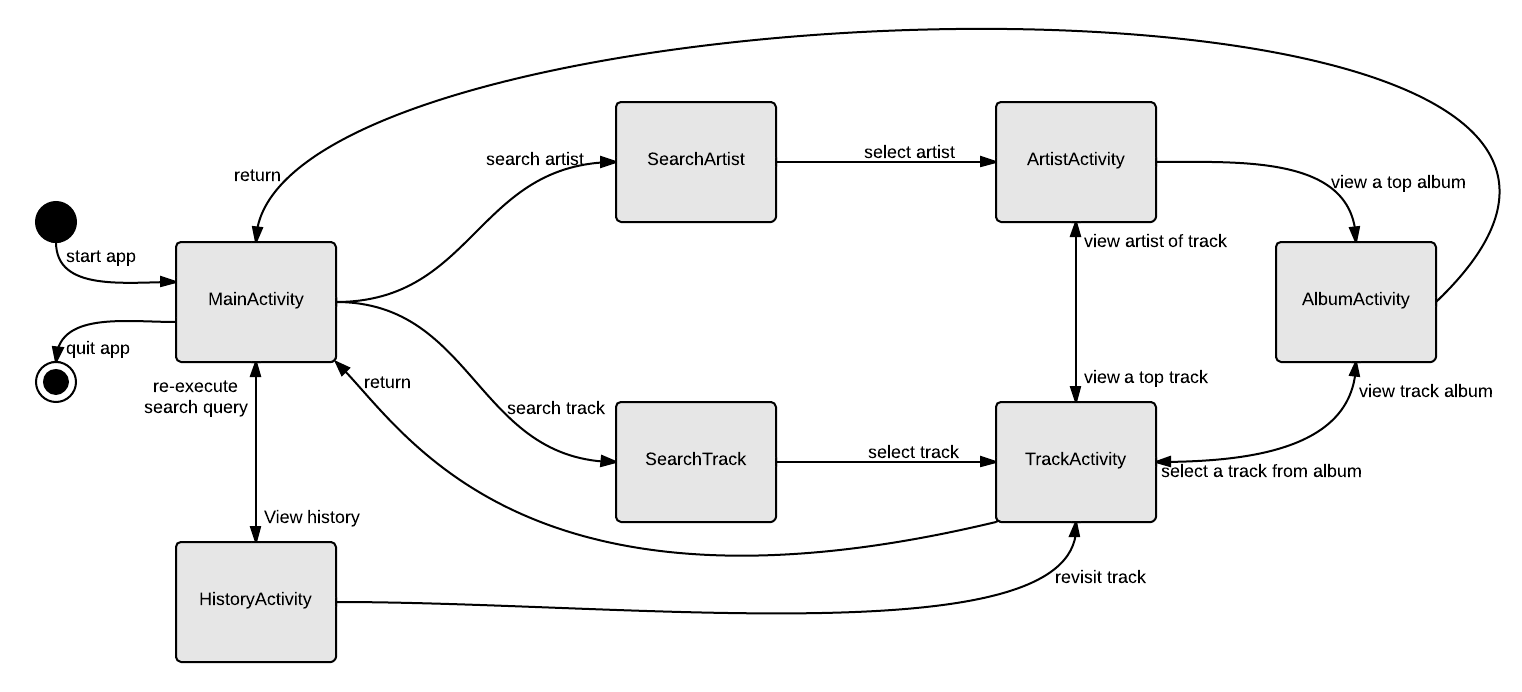
\includegraphics[scale=1]{Pictures/Dataflow2.png} \newline
	\small \textit{Afbeelding \figID : De data flow tussen alle activies.} \\ \normalsize

	\subsection{Databases}
	Er zijn 2 databases in dit project. Een bij elke klant, op elk toestel met een AMuRate app, en een grote centrale database op een server ergens. De lokale databases houden enkel data bij van hun gebruiken, en de externe verzamelt de scores van iedereen. We zullen nu beide databases bespreken.
	
	\subsubsection{Lokale Database}
	De lokale database moet data bijhouden die offline geraadpleegd zou willen worden. Hiermee bedoelen we onder andere geschiedenis van de ingevoerde zoekopdrachten, bekeken liedjes en de laatst gegeven scores. Aangezien deze applicatie vooral beroep doet op een actieve internetverbinding, zal er niet meer dan dat opgeslagen worden. \\ \newline \newpage
	De lokale database bevat dus twee tabellen en de operaties op deze tabellen gebeuren d.m.v. adapters. Die adapters maken de brug tussen procedures als 'read-X-from-database' en SQLite statements (zoals "SELECT X FROM tablename"). Er bestaat 1 adapter per tabel. \newline
	 
	 \begin{itemize}
		\item Ratings table \newline
		\begin{tabular}{| l | l | l | }
		\hline
		 Naam		& Type		& Sleutel		\\
		 \hline 
		id 		& integer 	& primary key 	\\
		date 	& integer	& 				\\
		rating 	& float 	& 				\\
		mbid 	& text 		& 				\\
		title 	& text 		& 				\\
		artist 	& text 		& 				\\
		sync	& integer 	& 				\\
		\hline
		\end{tabular} \newline
		\small \textit{Tabel \tabID : Het model van de Rating tabel in de lokale database.} \\ \normalsize \newline
		%\tabID2{Testnewcommand}
		De laatste kolom in de tabel is een 'sync bit'. Dat betekent dat hij enkel de waarde 0 of 1 kan hebben. Wanneer hij waarde 0 nul heeft, betekent het dat de score nog niet verzonden is naar de externe database. Dit kan voorvallen als er slechte verbinding is, of de server even uit zou staan bijvoorbeeld.  De DatabaseSyncer zal de score opsturen eens er terug verbinding is en de sync bit op waarde 1 zetten, zodat we weten dat hij opgestuurd is.
		
		\item Geschiedenis table \newline
		\begin{tabular}{| l | l | l | }
		\hline
		 Naam		& Type		& Sleutel		\\
		 \hline
		 id 	& integer 	& primary key 	\\
		 key	& integer	&				\\
		date 	& integer 	& 				\\
		artist 	& text 		& 				\\
		title 	& text 		& 				\\
		mbid 	& text 		& 				\\
		\hline
		\end{tabular} \newline
		\small \textit{Tabel \tabID : De Geschiedenis tabel in de lokale database.} \\ \normalsize
	
		Het enige wat ik kan verduidelijken over deze tabel is de 'key' in kolom 2. Deze gaat onderscheid maken tussen een zoek-geschiedenis-record en een track-viewed-geschiedenis. Deze twee soorten records staan samen in 1 tabel omdat ze toch bijna alle velden hetzelfde hebben. Enkel bij track-viewed-geschiedenis gaan we de MBID mee opslagen om sneller de informatie terug te kunnen downloaden.
	 \end{itemize}
	
\newpage
	\subsubsection{Externe Database}
	\label{sec:Extdb}
	De externe database moet enkel scores van gebruikers verzamelen. Om verschillende gebruikers te onderscheiden zal de er een user ID bijgehouden worden. De tabel zal er dan zo uitzien: \\ \newline
		\begin{tabular}{| l | l | l | }
		\hline
		 Naam		& Type		& Sleutel		\\
		 \hline 
		 idRatings 	& integer 	& primary key 	\\
		 MBID 		& text 		& 				\\
		 Artist		& text 		& 				\\
		 Title 		& text 		& 				\\
		 Rating		& float 	& 				\\
		 Date 		& integer 	& 				\\
		 User		& text 		& 				\\
		\hline
		\end{tabular}
	
	\small \textit{Tabel \tabID : De Rating tabel layout van de database op de server.} \\ \normalsize
		
		
	
\newpage % hack for layout	

	%%%%%%%%%%%%%%%
	% GUI SECTION %
	%%%%%%%%%%%%%%%
\section{GUI}
	Hieronder volgen enkele schermopnames van de uiteindelijke GUI. Deze opnames zijn van een echte Android telefoon genomen.  \\ \newline
	\hspace*{-5pt}\makebox[\linewidth][c]{%
	\begin{tabular} {p{7cm} >{\centering\arraybackslash}p{7cm}@{\hskip 0.5in}} %{>{\arraybackslash}m{7cm} >{\arraybackslash}m{7cm}} %{p{7cm} | p{7cm}}
		\centering 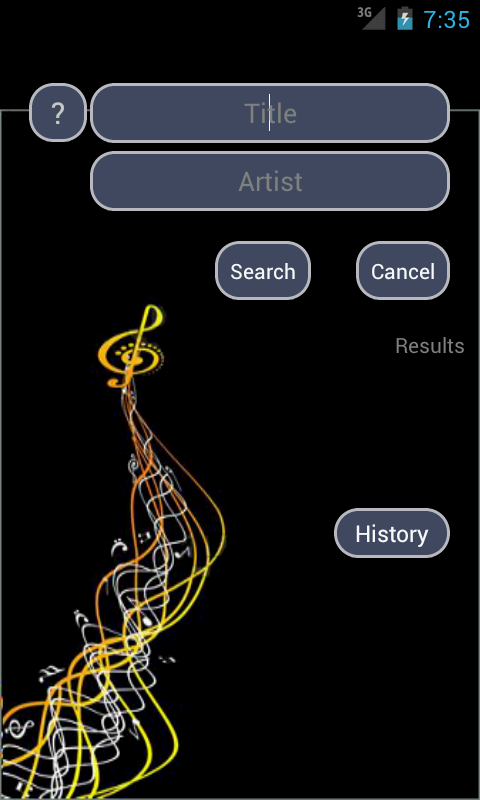
\includegraphics[scale=0.28]{Pictures/device-2013-05-25-213538.png}
		&  
		 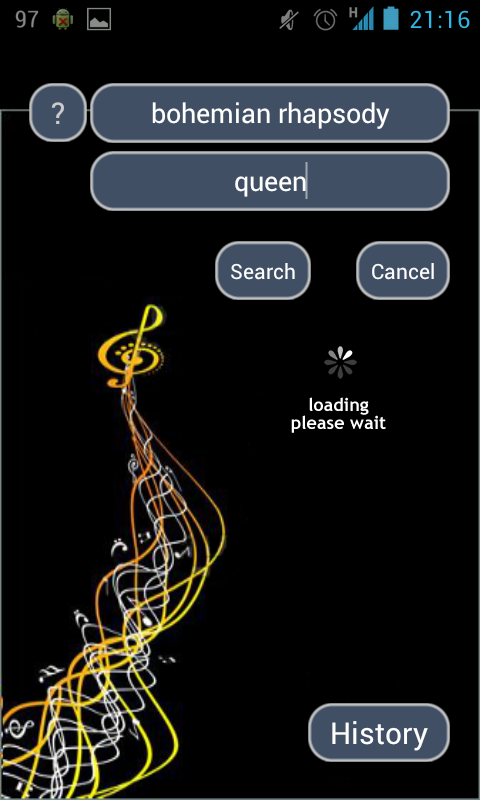
\includegraphics[scale=0.28]{Pictures/Screenshot_2013-05-24-21-16-07.png} 
		\\
		
		\centering \small \textit{Afbeelding \figID : Start scherm.}  \normalsize
		&  \small \textit{Afbeelding \figID : Zoek- en downloadproces.} \\  \normalsize
		
		\vspace{1pt} & \vspace{1pt} \\
		
\multicolumn{1}{p{7cm}|}{%		
			Dit scherm is het start scherm en het eerste wat de gebruiker ziet wanneer de applicatie gestart wordt. Er zijn twee velden om zoektermen in te geven (een voor artiest en een voor titel). De linkerboven knop met het vraagteken erop toont de instructies van de applicatie. De submit knop start een zoekopdracht, wanneer er zoektermen opgegeven zijn. De cancel knop wist alle ingevulde gegevens. }
&	
\multicolumn{1}{p{7cm}}{%
	% Zoek- en downloadproces &
			In het bovenstaande scherm werden de zoektermen "Bohemian Rhapsody" en "Queen" ingevuld, en op de zoekknop geklikt. De applicatie heeft de zoektermen verwerkt en start het informatie download proces. Een spinner met "Loading..." verschijnt op het scherm om de gebruiker te laten weten dat de applicatie aan het downloaden bezig is. }
\\	\end{tabular} 
} \newline

%%%%%%%%%%%%%%second graphics
\hspace*{-5pt}\makebox[\linewidth][c]{%
	\begin{tabular} {p{7cm} >{\centering\arraybackslash}p{7cm}@{\hskip 0.5in}} 
		\centering 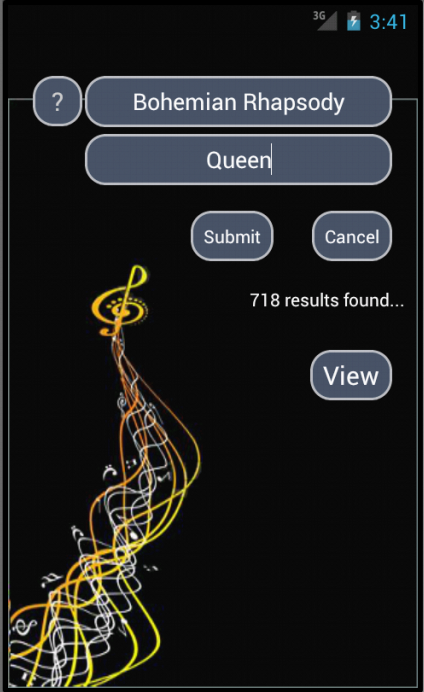
\includegraphics[scale=0.4]{Pictures/GUI_0124_startresults.png}
		& 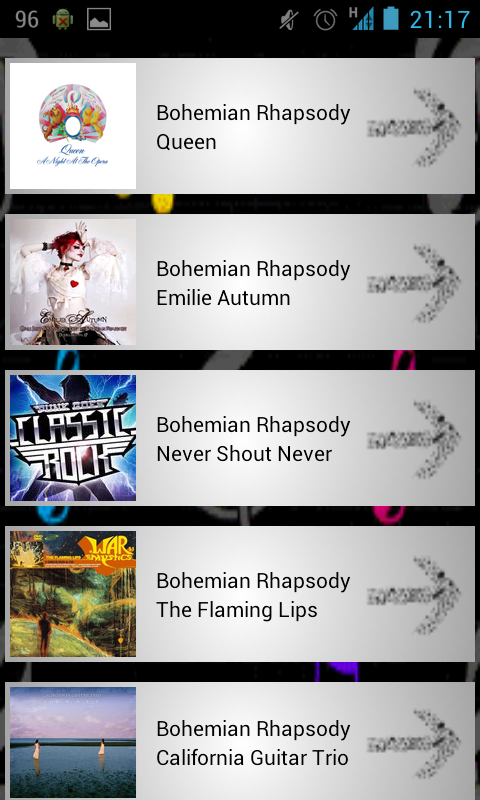
\includegraphics[scale=0.26]{Pictures/Screenshot_2013-05-24-21-17-57.png} \\
		
		\centering \small \textit{Afbeelding \figID : Klaar met downloaden.}  \normalsize
		&  \small \textit{Afbeelding \figID : Lijst met alle zoekresultaten.} \\  \normalsize
		\vspace{1pt} & \vspace{1pt} \\
		
\multicolumn{1}{p{7cm}|}{%%Klaar met downloaden \\	
			Wanneer de applicatie klaar is met het antwoord van de server te downloaden, verandert de text "Loading..." in het resultaat van de oproep, en het aantal gevonden resultaten. Wanneer er een positief aantal resultaten gevonden werd, verschijnt de knop View, waar de gebruiker op kan klikken om de resultaten te bekijken en het gewenste item te selecteren.
 } & \multicolumn{1}{p{7cm}}{%
	% Geeft alle resultaten weer &
			De lijst die resultaten weergeeft. Men kan op elke optie klikken om naar een pagina te gaan met meer informatie. Opties die niet beschikken over een afbeelding krijgen de standaard "Niet beschikbaar" afbeelding. De anderen worden asynchroon gedownloaded.
} \\ \end{tabular}
} \newline
%%%%%%%%%%%%%%%%%%%%%%%%%%%%%%%%%%%%
%%%%%%%%%%%%%%third graphics
\hspace*{-5pt}\makebox[\linewidth][c]{%
	\begin{tabular} {p{7cm} >{\centering\arraybackslash}p{7cm}@{\hskip 0.5in}} 
		\centering 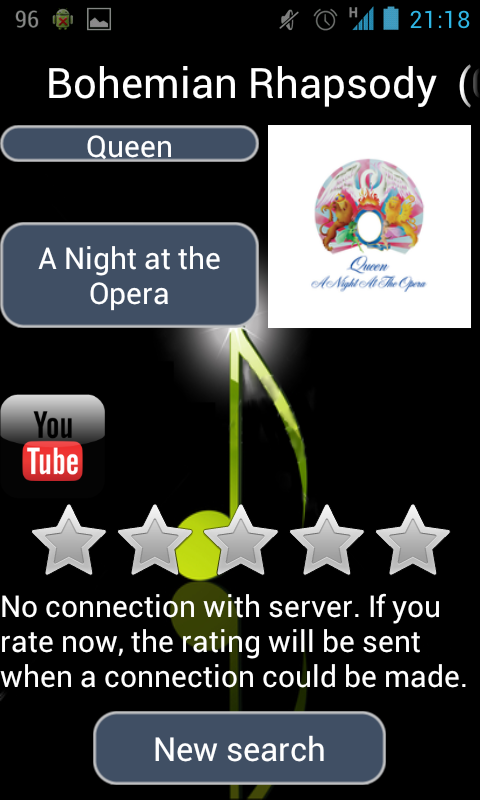
\includegraphics[scale=0.28]{Pictures/Screenshot_2013-05-24-21-18-48.png}
		& 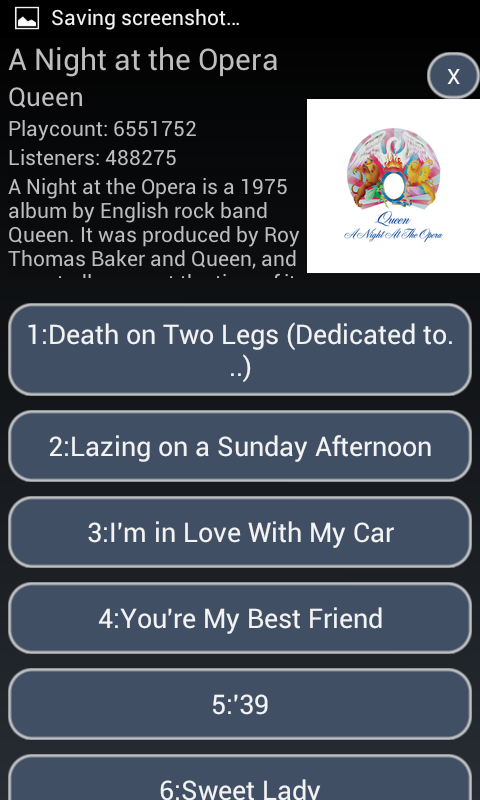
\includegraphics[scale=0.28]{Pictures/Screenshot_2013-05-24-21-20-57.png} \\
		
		\centering \small \textit{Afbeelding \figID : Gedetailleerd scherm van een lied.}  \normalsize
		&  \small \textit{Afbeelding \figID : Gedetailleerd scherm voor een album.} \\  \normalsize
		\vspace{1pt} & \vspace{1pt} \\
		
\multicolumn{1}{p{7cm}|}{%%Weergave van een track \\	
			Dit scherm geeft de gedetailleerde pagina van een individueel lied weer. De duratie van het lied wordt getoond, het album van het lied, een afbeelding en het score systeem. Het gemiddelde en het aantal van alle stemmen voor dat lied wordt getoond, en 5 sterren bieden de mogelijkheid aan de gebruiker om een eigen score aan het lied toe te dienen. Helemaal onderaan de knop om een nieuwe zoekopdracht te starten. Wanneer men op de youtube knop klikt zal de lokale youtube app starten. Wanneer de tekst en duratie te lang wordt voor het scherm, zal de tekst als marquee bewegen.
 } & \multicolumn{1}{p{7cm}}{%Albumscherm
	Wanneer er meer album informatie beschikbaar is en de gebruiker klikt op het album, komt hij op dit scherm terecht. Het bevat informatie over een gegeven album zoals artiest, albumafbeelding, playcount, listeners, een scrollbare album informatie tekst en alle liedjes die op dat album staan. De gebruiker kan op elk lied klikken om naar de gedetailleerde liedjes pagina te gaan. 
} \\ \end{tabular}
} \newline
%%%%%%%%%%%%%%%%%%%%%%%%%%%%%%%%
%%%%%%%%%%%%%%fourth graphics
\hspace*{-5pt}\makebox[\linewidth][c]{%
	\begin{tabular} {p{7cm} >{\centering\arraybackslash}p{7cm}@{\hskip 0.5in}} 
		\centering 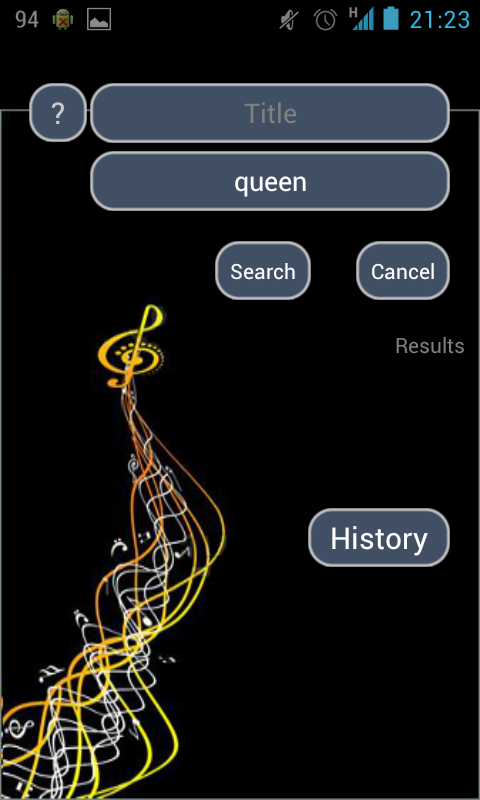
\includegraphics[scale=0.28]{Pictures/Screenshot_2013-05-24-21-23-29.png}
		& 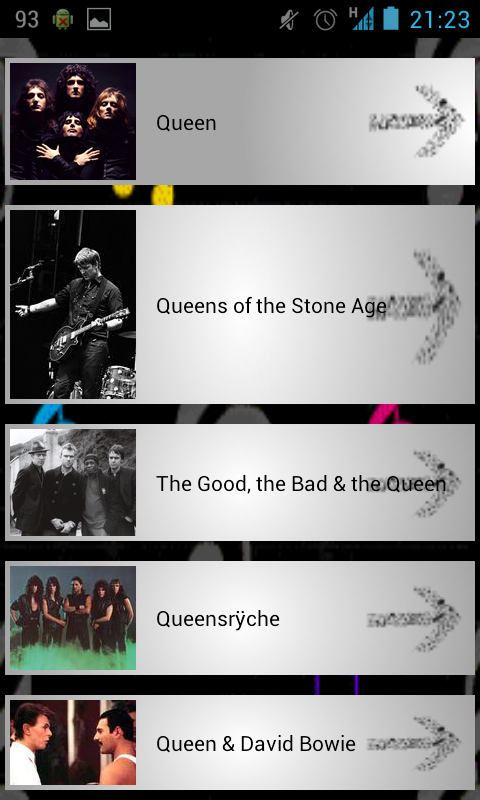
\includegraphics[scale=0.28]{Pictures/Screenshot_2013-05-24-21-23-51.png} \\
		
		\centering \small \textit{Afbeelding \figID : We willen hier enkel op artiestnaam zoeken.}  \normalsize
		&  \small \textit{Afbeelding \figID : Gevonden artiest resultaten voor querie.} \\  \normalsize
		\vspace{1pt} & \vspace{1pt} \\
		
\multicolumn{1}{p{7cm}|}{%%
	Als we enkel het artiest veld invullen, zal er een oproep gedaan worden naar de Last.fm API om artiesten te zoeken, niet tracks. Zoals normaal verschijnt de knop 'View' als er resultaten gevonden zijn, of verschijnt er een boodschap dat er geen matches waren voor de opgegeven zoekstring.
 } & \multicolumn{1}{p{7cm}}{%
 	De ArtistSearchActivity is zeer gelijkaardig aan de zoek tracks pagina. We tonen een afbeelding om te helpen kiezen welke artiest de gebruiker wou bezoeken.
} \\ \end{tabular}
} \newline
%%%%%%%%%%%%%%%%%%%%%%%%%%%%%%%%%%%%
%%%%%%%%%%%%%%fifth graphics
\hspace*{-5pt}\makebox[\linewidth][c]{%
	\begin{tabular} {p{7cm} >{\centering\arraybackslash}p{7cm}@{\hskip 0.5in}} 
		\centering 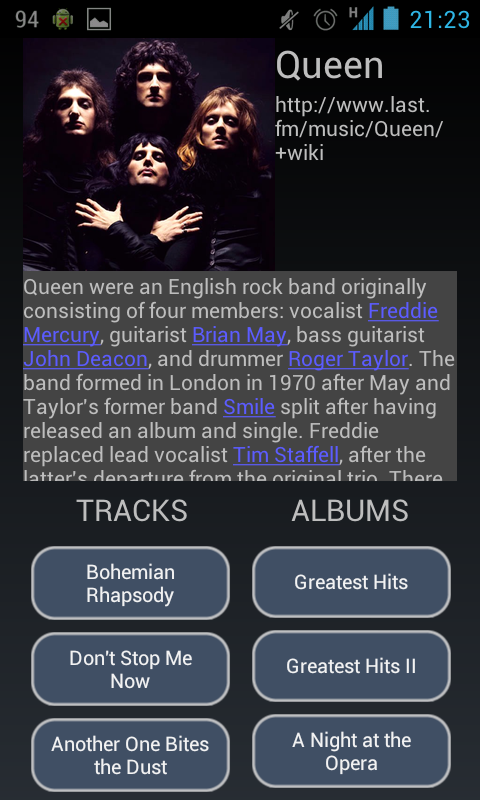
\includegraphics[scale=0.28]{Pictures/Screenshot_2013-05-24-21-23-02.png}
		& 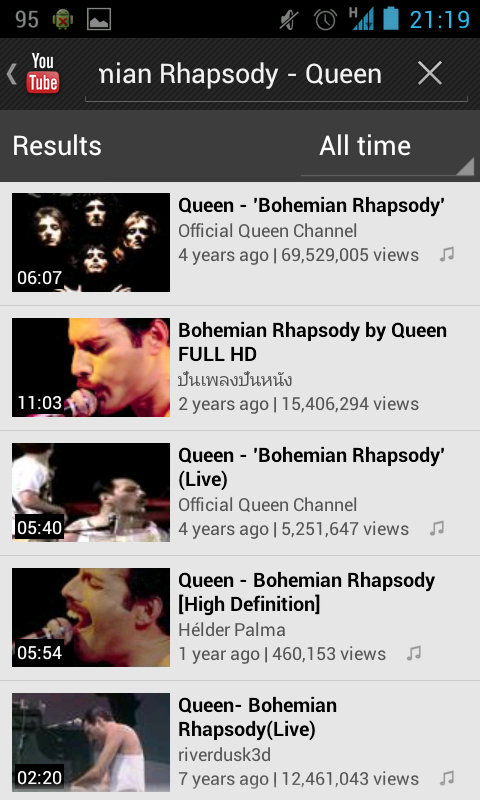
\includegraphics[scale=0.28]{Pictures/Screenshot_2013-05-24-21-19-44.png} \\
		
		\centering \small \textit{Afbeelding \figID : Gedetailleerd scherm van een artiest.}  \normalsize
		&  \small \textit{Afbeelding \figID : Link naar de youtube app.} \\  \normalsize
		\vspace{1pt} & \vspace{1pt} \\
		
\multicolumn{1}{p{7cm}|}{%%
	Wanneer een gebruiker meer informatie wilt over een artiest of groep, komt hij/zij op dit scherm terecht. Er is een link naar de wiki (als die bestaat), een scrollbare biografie, en een lijst van de artiest's top tracks en top albums. Men kan in beide lijsten scrollen en op elke item klikken om naar de gedetailleerde track/album pagina te gaan.
 } & \multicolumn{1}{p{7cm}}{%
 	Wanneer iemand in de TrackActivity op de youtube knop klikt, zal de lokale youtube app opgeroepen worden met als zoekterm de artiest en titel van het lied, zodat de gebruiker het liedje nog eens kan afspelen voordat hij/zij een score wilt bedelen.
} \\ \end{tabular}
} \newline
%%%%%%%%%%%%%%%%%%%%%%%%%%%%%%%%%%%%
%%%%%%%%%%%%%%six graphics
\hspace*{-5pt}\makebox[\linewidth][c]{%
	\begin{tabular} {p{7cm} >{\centering\arraybackslash}p{7cm}@{\hskip 0.5in}} 
		\centering 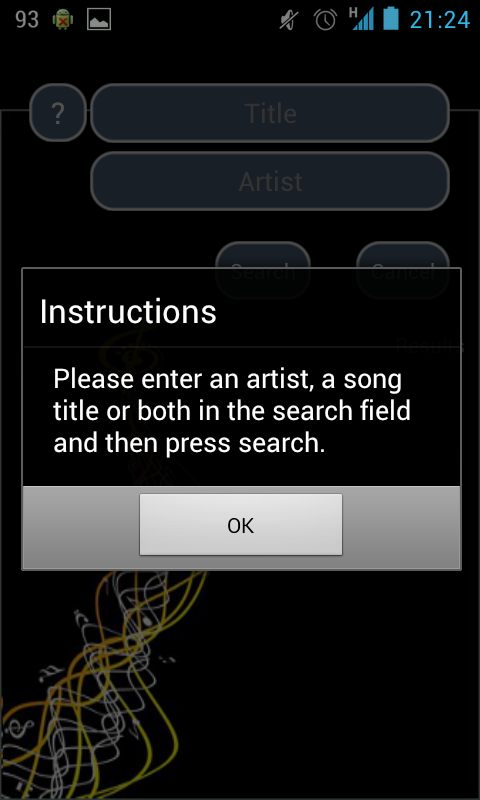
\includegraphics[scale=0.28]{Pictures/Screenshot_2013-05-24-21-24-20.png}
		& 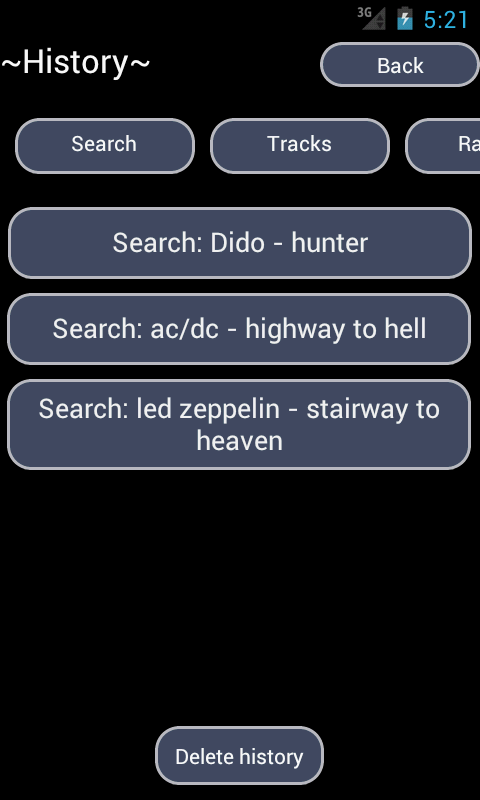
\includegraphics[scale=0.37]{Pictures/device-2013-05-26-192153.png} \\
		
		\centering \small \textit{Afbeelding \figID : Instructie pop up.}  \normalsize
		&  \small \textit{Afbeelding \figID : Geschiedenis scherm.} \\  \normalsize
		\vspace{1pt} & \vspace{1pt} \\
		
\multicolumn{1}{p{7cm}|}{%%
	Als men op het vraagteken in de linksboven hoek klikt, komt deze pop-up tevoorschijn. Het geeft de instructies die nodig zijn om een eerste zoekopdracht uit te voeren.
 } & \multicolumn{1}{p{7cm}}{%
 	Dit is het geschiedenis scherm. Vanboven is er een knop om terug te keren naar het hoofdscherm en er vlak onder enkele tabs. De tabs zitten in een horizontale scrollbar en kunnen dus verschoven worden. Wanneer de gebruiker op een van deze tabs klikt, worden de respectievelijke geschiedenis records in het midden ingeladen. Met de onderste knop kan de gebruiker deze records wissen. Op dit scherm zien we de 'search' geschiedenis. Door op een item te klikken worden die zoektermen terug ingevuld in de zoekvelden.
} \\ \end{tabular}
} \newline
%%%%%%%%%%%%%%%%%%%%%%%%%%%%%%%%%%%%
%%%%%%%%%%%%%%seven graphics
\hspace*{-5pt}\makebox[\linewidth][c]{%
	\begin{tabular} {p{7cm} >{\centering\arraybackslash}p{7cm}@{\hskip 0.5in}} 
		\centering 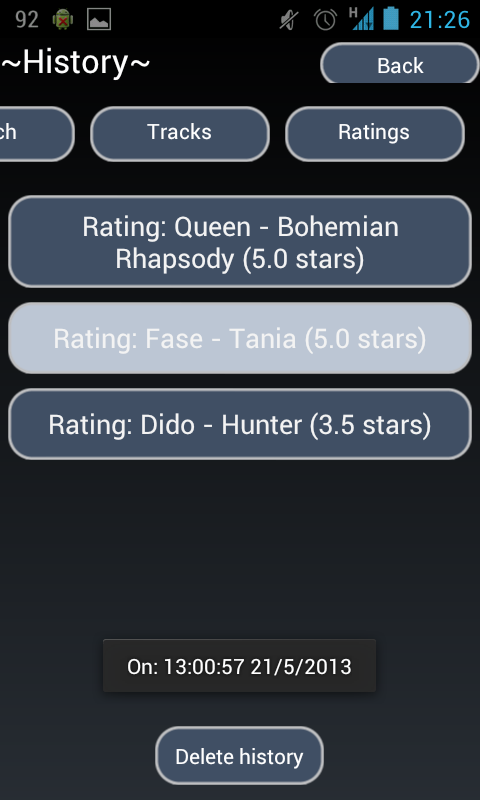
\includegraphics[scale=0.28]{Pictures/Screenshot_2013-05-24-21-26-47.png}
		& 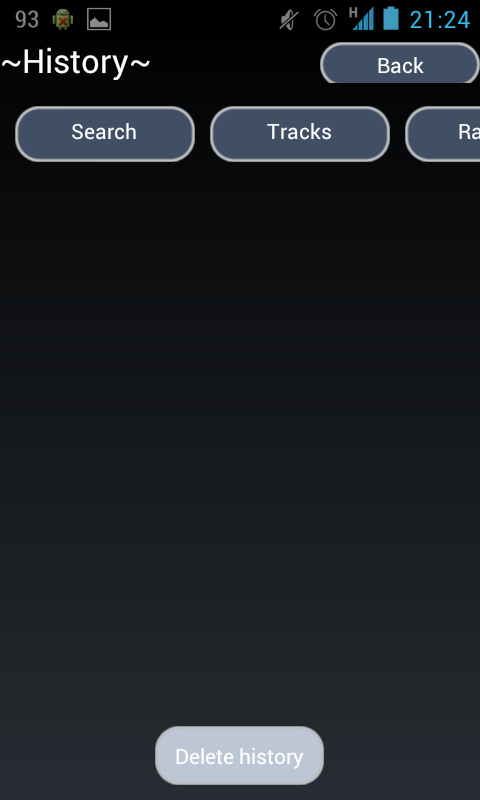
\includegraphics[scale=0.28]{Pictures/Screenshot_2013-05-24-21-24-56.png} \\
		
		\centering \small \textit{Afbeelding \figID : Geschiedenis ratings.}  \normalsize
		&  \small \textit{Afbeelding \figID : Geschiedenis gewist.} \\  \normalsize
		\vspace{1pt} & \vspace{1pt} \\
		
\multicolumn{1}{p{7cm}|}{%%
	Deze tab geeft een overzicht van alle gegeven scores. We tonen de titel, artiest en aantal gegeven sterren. Door op een score te klikken verschijnt er een Toast die zegt wanneer die rating precies gegeven werd.
 } & \multicolumn{1}{p{7cm}}{%
 	Delete history verwijdert de geschiedenis records van de huidig geopende tab.
} \\ \end{tabular}
} \newline
%%%%%%%%%%%%%%%%%%%%%%%%%%%%%%%%%%%%
% history gui
	
	
\newpage %hack for layout
%%%%%%%%%%%%%%%%%%%%%%%%%
%%	Technische details %%
%%%%%%%%%%%%%%%%%%%%%%%%%
\section{Technische details}
	\subsection{Data collection}
	De AMuRate data collection server is een combinatie van een Java server en een MySQL database, die momenteel lokaal op mijn laptop draaien. Die externe database bevat één grote tabel, zoals hier \ref{sec:Extdb} te zien is. Wanneer een score gegeven zou worden op de applicatie, stuurt die de score via sockets\footnote{Standaard communicatiemiddel tussen programmas en computerprocessen} naar de Java server. Wanneer die een verbinding binnen krijgt, wordt er een nieuwe thread aangemaakt (multithreading) die ook een socket verbinding gaat maken met de MySQL database op poort 3306. De database slaagt alle records bij op, tenzij er al een unieke combinatie bestaat (mbid+user).
	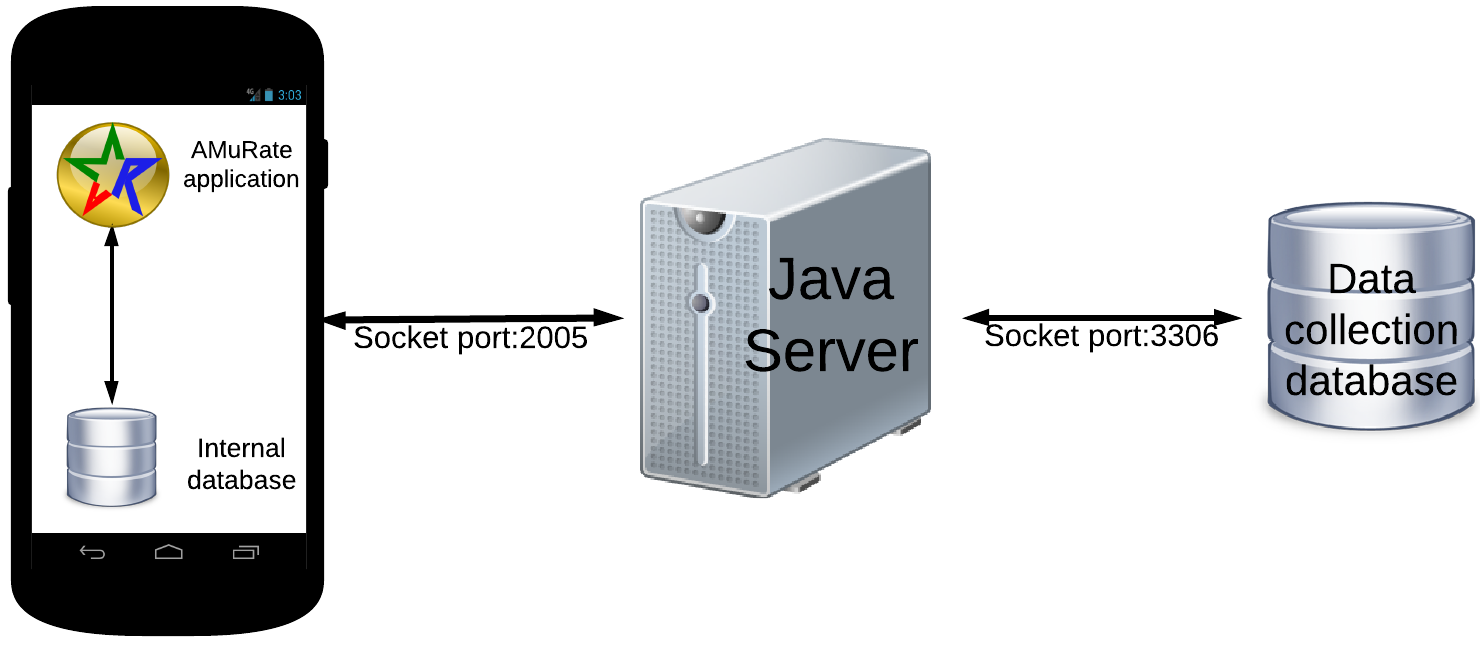
\includegraphics[scale=1]{Pictures/datacollection.png} \newline
	\small \textit{Afbeelding \figID : Overzicht van de score verbindingen.} \\ \normalsize

	\subsection{Unieke records}
	Gebruikers mogen maar 1 score per lied geven. Records in de database hebben dus 'MBID' en 'User' als primaire sleutel. Dit is deels om SPAM te voorkomen en deels om een eerlijke gemiddeldes te kunnen maken van scores. Wanneer een lied wordt geladen in de applicatie, wordt er in de databases gekeken of de gebruiker al een score heeft gegeven voor de MBID geassocieerd met het gekozen lied. Wanneer de gebruiker al een score heeft gegeven, zal hij/zij geinformeerd worden met de gegeven score. 
	Als er geen verbinding is met de externe database, kunnen we op die moment niet achterhalen of de gebruiker al eens een score heeft gegeven op dat lied. We slagen de score dan even lokaal op tot er terug een verbinding op stand kan komen en updateten dan de gegeven score. Zie sectie Database Syncing.
	
	\subsection{Verschillende zoekopdrachten}
	Op de homepagina zijn er twee inputvelden; 'artist' en 'title'. Gebruikers kunnen kiezen welke velden ze wel en niet willen/kunnen invullen om te vinden wat ze zoeken. Dat levert ons 4 opties;
		\begin{itemize}
			\item \textbf{artiest en geen titel} \\
		Aangezien er niets is ingevuld, kan er ook niets opgezocht worden. De gebruiker krijgt een boodschap te zien dat er minstens 1 veld ingevuld moet zijn. \\
		
			\item \textbf{Wel artiest en geen titel} \\
		Wanneer enkel de artiestnaam (of groepsnaam) ingevuld wordt, zal er een zoekopdracht gedaan worden naar alle artiesten/groepen met een gelijkaardige naam als de querie. Als er resultaten gevonden zijn, kan de gebruiker kiezen uit een lijst van resultaten. Wanneer een resultaat met een afbeeldingsurl kwam, kunnen we er een afbeelding bij tonen om het selectieproces te vergemakkelijken. Wanneer de gebruiker op een van de opties klikt zal hij doorgewezen worden naar de ArtistActivity pagina van die artiest/groep. \\
		
			\item  \textbf{Geen artiest en wel titel} \\
		Er wordt gezocht naar alle liedjes met een gelijkaardige titel als die van de querie. De artiesten kunnen varieren en worden niet gefilterd. Als er resultaten gevonden worden, kan de gebruiker op eender welke klikken om naar de TrackActivity te gaan, waar hij/zij een score kan geven.\\
				
			\item  \textbf{Wel artiest en wel titel} \\
		Wanneer beide velden ingevuld worden wordt er dezelfde aanvraag als hier net boven gestuurd naar de Last.fm API, maar in de querie voegen we de artiestnaam toe. De filtering gebeurt op de Last.fm API zelf, en indien er matches zijn voor beide gegevens, kan de gebruiker erop klikken om naar TrackActivity te gaan.
		\end{itemize}
		
	\subsection{Database Syncing}
	Het kan voorkomen dat de Java server of de MySQL database offline zijn voor een bepaalde onverwacthe periode/reden. Als de gebruiker een score wilt geven en de applicatie ziet dat er geen verbinding tot stand kan komen, wordt de score tijdelijk opgeslagen in de lokale database. Hier komt de kolom 'Sync' handig in voor, want we zetten die sync bit dan op 0 (unsynced. 1=synced). Telkens wanneer de gebruiker verwisselt tussen schermen in de applicatie (redelijk vaak dus), zal de DatabaseSyncer kijken of er unsynced scores in de lokale database zitten. (Dit gebeurt natuurlijk volledig op de achtergrond.) Wanneer er unsynced scores zijn, zal er gekeken of er nu wel een verbinding gemaakt kan worden. Zoniet proberen we laten wel opnieuw, zowel  gaan we ze een voor een opsturen naar de externe database. Wanneer ze allemaal zijn aangekomen zetten we hun sync bits op 1 (synced).
		
	
	\subsection{Uitbreidbaarheid}
	De uitbreidbaarheid van het systeem is zeer eenvoudig, in de veronderstelling dat de gebruiker wel enige voorkennis van Android development bezit. Om nieuwe functionaliteiten toe te voegen moeten er gewoon activities bijgemaakt worden, en toegevoegd worden in het Android Manifest.
	
	\subsection{Installatie}
	De applicatie staat nog niet in de Android Play Store, maar is wel gratis te downloaden en installeren op de AMuRate website (zie sectie Bronnen, tools en referenties). 
	\begin{itemize}
		\item Navigeer met de Android telefoon naar de AMuRate website 
		\item Klik op "Download .apk"
		\item Navigeer naar de Downloads map en dubbel klik op "AMuRate.apk"
		\item Op het AMuRate installatiescherm klik rechtsonder op "Install"
		\item Wanneer "Application installed" tevoorschijn komt kan je klikken op "Done" om het proces te sluiten, of "Open" om de applicatie direct te starten
	\end{itemize}
	
	\newpage
%%%%%%%%%%%%%%%%%%%%%%%%%%
% Tegengekomen problemen %
%%%%%%%%%%%%%%%%%%%%%%%%%%
\section{Tegengekomen problemen}

	\subsection{Synchronious tasks}
	Wanneer data binnengehaald moet worden van de API, mag die operatie niet gebeuren op de main thread van het programma, anders zal de applicatie zeer traag/onbruikbaar zijn elke keer dat er iets gedownloaded moet worden. Hierom werd een klasse "MyConnection" gemaakt, die async\footnote{Asynchronous betekent dat een process tegelijkertijd naast een ander process kan werken.} data begint binnen te laden terwijl de applicatie vloeiend kan blijven voortdraaien.
	
	\subsection{Tracks omzetten van verschillende representaties}
	Een tegengekomen probleem in dit project, is dat de Last.fm API oproepen (zoals track.getinfo en track.search) antwoorden met verschillende representaties. Om een voorbeeld te geven: hieronder bevinden zich de resultaten van twee oproepen naar methoden voor het lied 'Bohemian Rhapsody' van Queen. Er kan opgemerkt worden dat in het eerste resultaat 'artist' een top level attribuut is van 'track'. In het tweede snippet is 'artist' opnieuw een object met zijn eigen velden. Om zo een object\footnote{In dit document gebruik ik XML notatie omdat deze makkelijker leesbaar is, maar in de broncode wordt er enkel met JSON gewerkt.} om te zetten in een 'Track' klasse, moet de Track klasse een onderscheid maken in wat voor soort object gebruikt wordt om de klasse te initialiseren. De beste oplossing hiervoor is om per representatie een loadFromX functie te maken die weet hoe X eruit ziet en waar alle informatie staat. \\
	
	Track.search resultaat:\\
	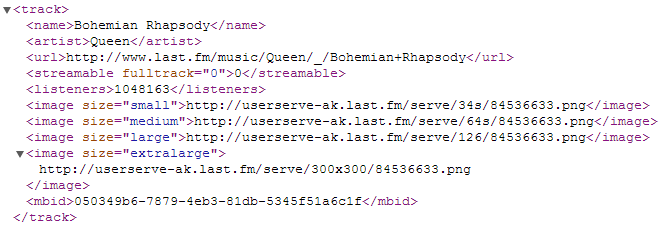
\includegraphics[width=15cm]{Pictures/track_search.png} \\ \newline
	\small \textit{Afbeelding \figID : Resultaat van Track.search GET voor Bohemian Rhapsody - Queen.} \\

	Track.getinfo resultaat: \\
	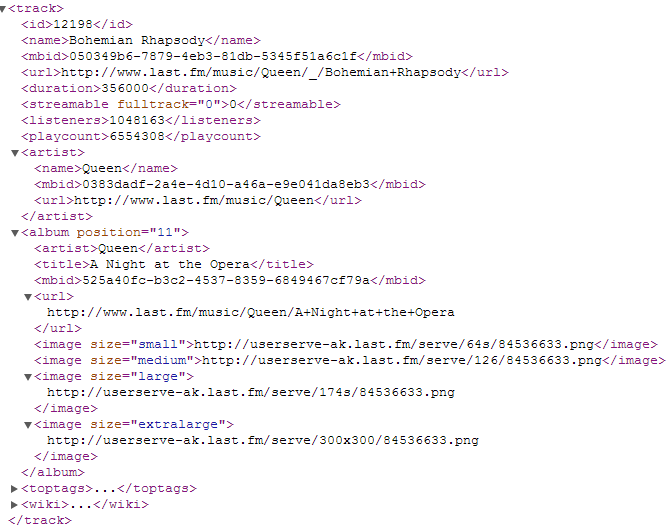
\includegraphics[width=15cm]{Pictures/track_getinfo.png}\\ \newline
	\small \textit{Afbeelding \figID : Resultaat van Track.getinfo GET voor Bohemian Rhapsody - Queen.}
		


	
\newpage	
\section{Bronnen, tools en referenties}

	\begin{itemize}
		
	\item \textbf{Eclipse} \\
	Programmeerplatform Eclipse (Juno) werd gebruikt voor de implementatie en emulatie.	\\
	\url{http://www.eclipse.org/}

	\item \textbf{Android Development Toolkit (ADT)} \\
	Deze plug-in bevat alle benodigdheden om programma's voor Android in Eclipse te bouwen en testen.\\
	\url{http://developer.android.com/sdk/index.html}
	
	\item \textbf{MySQL} \\
	Op MySQL workbench werd de data collection aangemaakt en kon de luisterende socket aangemaakt worden. \\
	\url{http://www.mysql.com/}	
	
	\item \textbf{LucidChart} \\
	Op deze website werden de diagrammen en andere afbeeldingen in dit document gegenereerd.\\
	\url{lucidchart.com}
	
	\item \textbf{AMuRate homepagina} \\
		\url{http://dsverdlo.github.com/AMuRate}
		
	\item \textbf{Android} \\
		\url{http://www.android.com/}
		
	\item \textbf{Ice Cream Sandwich} \\
		\url{http://www.android.com/about/ice-cream-sandwich/}	
		
	\item \textbf{Last.fm} \\
		\url{http://www.last.fm/home}	
		
	\item \textbf{Github} \\
		\url{https://github.com/}



	\end{itemize}



\end{document}
